%!TeX root=../tese.tex
%("dica" para o editor de texto: este arquivo é parte de um documento maior)
% para saber mais: https://tex.stackexchange.com/q/78101/183146

% Os capítulos de compõem a dissertação/tese, com numeração normal, podem
% ser inseridos diretamente aqui ou "puxados" de outros arquivos.
% Em alguns (raros) casos, pode ser interessante usar \include ao
% invés de \input: https://tex.stackexchange.com/a/32058/183146
%!TeX root=../tese.tex
%("dica" para o editor de texto: este arquivo é parte de um documento maior)
% para saber mais: https://tex.stackexchange.com/q/78101/183146

%% ------------------------------------------------------------------------- %%
\chapter{Introdução}
\label{cap:introducao}

Com a variedade de serviços oferecidos pela internet, a quantidade de requisições
que são feitas a um servidor web aumenta. De acordo com \cite{facebook:topProblems}, o Facebook em 2014 recebia
uma quatidade de consultas da ordem de bilhões por segundo. Nesse sentido é esperado que
também aumente o número de requisições maliciosas, como por exemplo SQL injection que está 
no top 10 da OWASP \cite{owasp:top10}, uma organização sem fins lucrativos que visa melhorar a segurança em 
softwares, através da publicação de artigos, metodologias e documentação de maneira gratuita.

Em tal cenário se faz necessário um sistema automático de detecção de requisições maliciosas, pois analisar cada
uma delas manualmente pode ser inviável ou bastante custoso. Uma possível solução é criar modelos de aprendizagem
de máquina para encontrar padrões de requisições maliciosas e então tomar decisões automatizadas com base no
resultado desses modelos.

Além disso, é desejável que esse projeto tenha um custo baixo em termos financeiros, de rede e
de consumo de energia. Para isso, se tem proposto o uso de hardware de baixo custo para implantação 
desse tipo de sistema. Em \cite{sbrc_estendido:lucas} há uma análise que conclui que é possível usar Raspberry Pi como nó de
um cluster de processamento de dados.

\subsection{Objetivo}

O objetivo deste conclusão de curso é construir modelos de aprendizagem de máquina para classificar
requisições maliciosas. Tais modelos utilizam logs de servidores HTTP para detectar potenciais ataques
de SQL Injection e XSS. E por fim, rodar esses modelos em Raspberry Pi.

Portanto, avançar o que foi realizado no TCC “Análise de Desempenho de Computadores de Baixo Custo em um Sistema de 
Detecção de Intrusão” de Lucas Seiki Oshiro \cite{tcc:lucas}.

\subsection{Resultado alcançados}

Aqui vem os resultados alcançados

\subsection{Organização da monografia}

Os próximos capítulos desta monografia estão dividos da seguinte maneira: 

\begin{itemize}
    \item Capítulo 2: Trabalhos relacionados a este TCC e resultados encontrados.
    \item Capítulo 3: Conceitos e ferramentas que foram usados.
    \item Capítulo 4: Ambiente usado e como os dados foram coletados.
    \item Capítulo 5: Como o modelo final foi selecionado.
    \item Capítulo 6: Metodologia e os resultados dos experimentos.
    \item Capítulo 7: Conclusão.
    \item Capítulo 8: Avaliação pessoal e crítica.
\end{itemize}
\par

%!TeX root=../tese.tex
%("dica" para o editor de texto: este arquivo é parte de um documento maior)
% para saber mais: https://tex.stackexchange.com/q/78101/183146

%% ------------------------------------------------------------------------- %%
\chapter{Revisão da literatura}
\label{cap:fundamentation}

O uso de modelos de aprendizagem de máquina para detectar intrusões em servidores HTTP 
por meio de logs já foi estudado em outros trabalhos. Abaixo cito os artigos que nos
serviram de referência e qual modelo foi utilizado.

\begin{itemize}
    \item \cite{ref:art3}: este trabalho analisa uma fase anterior dos ataques HTTP, a etapa
    de exploração de vulnerabilidades. Nessa etapa, em geral, um crawler pode ser executado 
    em busca de possiveis vulnerabilidades, e nesse sentido o proceso distinguir tais 
    requisições das requisições de usuários ajuda na prevenção de ataques. Para isso, o 
    trabalho propos regras estabelecidas manualmente após uma análise dos logs, isto é, 
    nenhum modelo de aprendizagem de máquina tradicional foi usado.

    \item \cite{ref:art6}: este trabalho visa detectar atividades maliciosas no ambiente 
    da nuvem. Uma vez que sua adoção vem crescendo, a supercie de ataque cresce propocionalmente.
    Nesse sentido, o trabalho propõem analisar arquivos de logs gerados pela nuvem e por aplicações
    web para treinar modelos de aprendizagem de máquina e automatizar a sua deteccção. Para isso
    usou modelo de árvore de decisão e redes neurais.

    \item \cite{ref:art2}: similar aos trabalhos anteriores, este trabalho propõe automatizar
    a detecção de ataques utilizando aprendizagem de máquina, contúdo, neste trabalho
    o foco principal é o SQL injection motivado pela grave falta de privacidade 
    que esta falha pode proporcionar. Rara isso propõe um modelo de naive bayes.
\end{itemize}

Observar estes trabalhos direcionou a pesquisa no sentido de que os modelos de 
aprendizagem de máquina podem ser utilizados para detectar falhas de segurança
em servidores HTTP, além disso qual modelo avaliar, e por fim quais dados foram utilizados.

Vale deixar registrado, um agradecimento ao autor Jaron Fontaine do trabalho \cite{ref:art6}, que gentilmente
indicou quais logs reais foram usados em seu trabalho e onde encontrá-los.
\par

%!TeX root=../tese.tex
%("dica" para o editor de texto: este arquivo é parte de um documento maior)
% para saber mais: https://tex.stackexchange.com/q/78101/183146

%% ------------------------------------------------------------------------- %%
\chapter{Conceitos}
\label{cap:concepts}

Este capítulo visa apresentar os conceitos que foram utilizados para o desenvolvimento deste TCC. Serão apresentadas as ferramentas utilizadas para realizar o ETL, simular os logs de ataques, modelos que foram utilizados e por fim quais frameworks usados para o aprendizado de máquina.

\section{Ferramentas}

\begin{description}
    \item[Kali Linux] \hfill \\ 
        O Kali Linux é uma distribuição linux open source baseada em Debian. Tem como foco auxiliar em tarefas relacionada a segurança da informação e testes de penetração.
    \item[xsser] \hfill \\ 
        O xsser é um utilitário que está instalado por padrão no kali linux. Sua função é automatizar a deteccão, exploração e análise de ataques XSS em aplicações web.
    \item[sqlmap] \hfill \\ 
        O sqlmap é um utilitário que está instalado por padrão no kali linux. Sua função é automatizar a detecção e exploração de ataque de SQL injection em aplicações web.
    \item[Pandas] \hfill \\ 
        O Pandas é uma ferramenta  em python para o processo de análise de dados, especificamente neste trabalho, foi utilizado para realizar o ETL e analise dos logs coletados.
    \item[DVWA] \hfill \\ 
        DVWA é uma aplicação web com falhas de segurança conhecidas que podem ser exploradas no ambiente local e controlado, facilitando assim a simulação de ataques.
  \end{description}

\section{Modelos}


\begin{description}
    \item[Árvore de decisão] \hfill \\ Árvore de decisão é um modelo de representação dos dados que, neste trabalho, visa classificar os dados tendo como base um conjunto de atributos. \\ 
    Elas são construidas particionando os dados em conjuntos, chamados de nós, até que uma folha seja encontrada, está então é a classe do dados. Veja na imagem abaixo.
    
    \begin{figure}
        \centering
        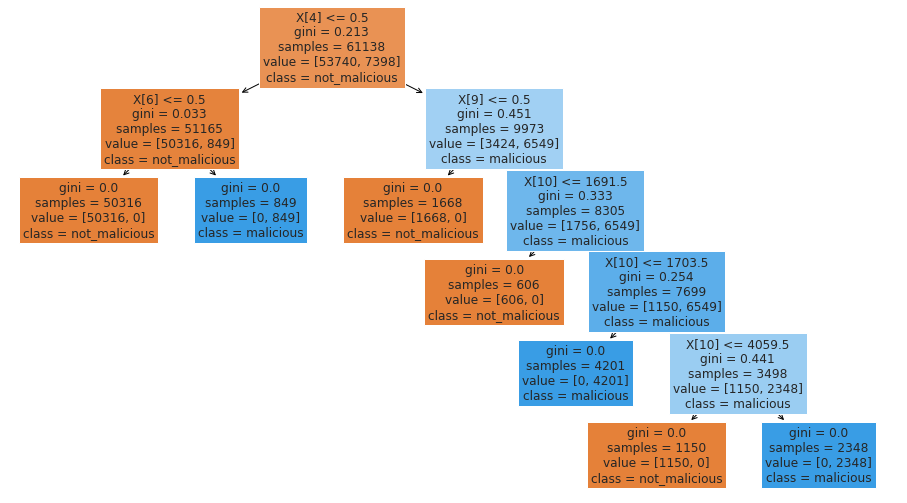
\includegraphics[width=.6\textwidth]{figuras/ex_decicion_tree.png}
        \caption{Exemplo de árvore de decisão.\label{fig:ex_decision_tree}}    
    \end{figure}

    Este modelo é útil pois a sua interpretabilidade é alta.

    \item[Florestas aleatórias] \hfill \\ Florestas aleatórias é um modele de aprendizagem de máquina de combina árvores de decisão. Isto é, uma certa quantidade de árvores são treinadas de maneira independente uma da outra, utilizando diferentes partes do conjunto de dados. \\ 
    E para realizar a classificação, cada árvore realiza uma classificação (voto) e o resultado final da floresta é a classe com mais votos, como ilustrado na image abaixo:\\

    \begin{figure}
        \centering
        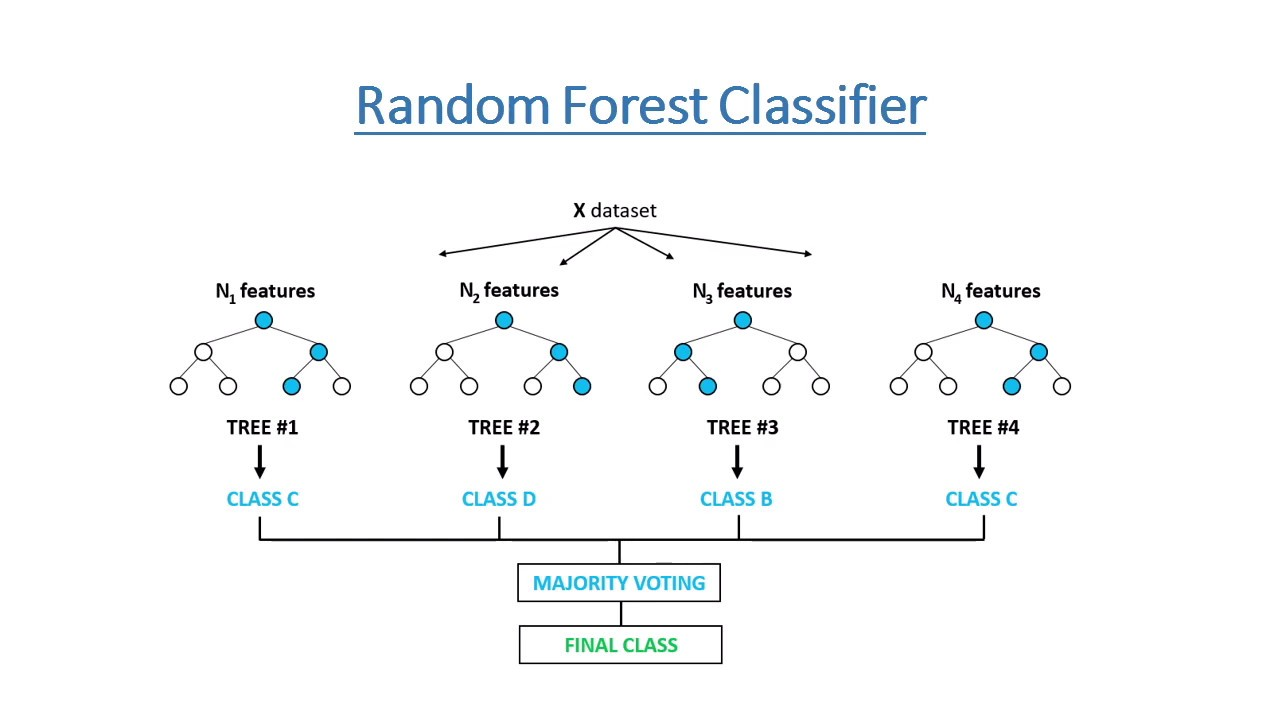
\includegraphics[width=.8\textwidth]{figuras/ex_random_forest.jpg}
        \caption{Exemplo de floresta aleatória.\label{fig:ex_random_forest}}    
    \end{figure}

    Este modelo possui dois pontos de atenção: sua interpretabilidade é baixa, dado o número de classificadores que temos que analisar, e também é consideravelmente mais pesado que o anterior, pois ele treina algumas árvores de decisão.
\end{description}

\section{Ferramentas de aprendizado de máquina}

\begin{description}
    \item[scikit-learn] \hfill \\ Scikit-learn é uma ferramenta que implementa algoritmos de aprendizagem de máquina, supervisionados e não supervisionados. Em particular, o modelo de árvore de decisão e floresta aletória.\\ 
    Além disso, ela integra com o ecossistema python, isto é: numpy, pandas e matplotlib. E também fornece uma interface sólida, que facilita o seu uso. 

    \item[Apache Spark] \hfill \\ Apache Spark é uma ferramenta para trabalhar com aprendizagem de máquina de maneira distribuida ou em um único nó. \\
    Assim como o scikit-learn, há alguns modelos implementados que estão pronto para ser utilizados, em particular, há implementações de árvore de decisão e floresta aleatória. \\
    Há suporte para algumas linguagens, como: Python, Scala, Java e R.
\end{description}
\par

%!TeX root=../tese.tex
%("dica" para o editor de texto: este arquivo é parte de um documento maior)
% para saber mais: https://tex.stackexchange.com/q/78101/183146

%% ------------------------------------------------------------------------- %%
\chapter{Ambiente e dados}
\label{cap:data}

Este capítulo mostra o ambiente que foi usado para realizar as simulações de ataque,
coletar os logs e treinar os modelos. Além disso, também será explicado como os logs 
foram coletados e processados.

Alguns dos itens foram inspirados no trabalho de conclusão de curso "Análise de 
Desempenho de Computadores de Baixo Custo em um Sistema de Detecção de Intrusão" de 
Lucas Seiki Oshiro \cite{tcc:lucas}.

O ambiente aqui mostrado pode ser visto na Figura \ref{fig:arquitetura_total}. Na máquina pessoal foram 
criadas duas máquinas virtuais para simular os ataques, o Google Colab 
usado para avaliar, treinar e compartilhar os modelos e por fim o Raspberry Pi e o Macbook 
para rodar os experimentos.

\begin{figure}
    \centering
    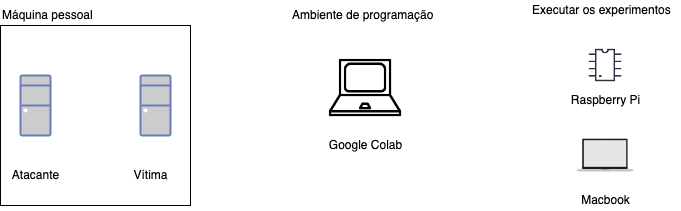
\includegraphics[width=1\textwidth]{figuras/arquitetura_total.png}
    \caption{Infraestrutura usada neste trabalho. \label{fig:arquitetura_total}}
\end{figure}


\section{Máquinas}

\subsection{Máquinas físicas}

Neste trabalho, duas máquinas físicas foram utilizadas: um desktop e um notebook, além do ambiente Google Colab. 

\begin{itemize}
    \item Máquina pessoal
        \begin{itemize}
            \item Sistema operacional: Ubuntu 20.04 LTS
            \item Processador: Intel i7-10700, 8 núcleos, 4,8 GHz
            \item Memória RAM: 32Gb
        \end{itemize}
        Esta máquina foi utilizada para iniciar duas máquinas virtuais que serão usadas 
        como o atacante e a vítima.
    \item Macbook 
        \begin{itemize}
            \item Sistema operacional: macOS Monterey - 12.0.1
            \item Processador: M1, 8 núcleos, 3,2 GHz
            \item Memória RAM: 8Gb
        \end{itemize}        
        Esta máquina foi utilizada para rodar os experimentos com Apache Spark, os quais 
        serão comparados com os resultados dos computadores de placa única.
\end{itemize}


\subsection{Máquinas virtuais}

Aqui estão as duas máquinas virtuais que foram usadas: o atacante e a vítima, como mostrada na Figura \ref{fig:arquitetura_ataque}. 
Elas foram criadas na máquina pessoal.

\begin{itemize}
    \item Atacante
        \begin{itemize}
            \item Sistema operacional: Kali Linux 2021.2
            \item Processador: Intel i7-10700, 4 núcleos, 4,8 GHz
            \item Memória RAM: 4Gb
        \end{itemize}
    \item Vítima
        \begin{itemize}
            \item Sistema operacional: Ubuntu 20.04 LTS
            \item Processador: Intel i7-10700, 4 núcleos, 4,8 GHz
            \item Memória RAM: 4Gb
        \end{itemize}        
\end{itemize}



\subsection{Computador de placa única}

Neste trabalho um Raspberry Pi foi utilizado, nele executamos as tarefas de treino e classificação
dos logs.

\begin{itemize}
    \item Raspberry Pi
        \begin{itemize}
            \item Sistema operacional: Raspberry Pi OS - 10.9
            \item Processador: Quad Core 1,2GHz Broadcom BCM2837
            \item Memória RAM: 1Gb
        \end{itemize}
\end{itemize}

\section{Ambiente de programação}
\begin{itemize}
    \item Google Colab
        \begin{itemize}
            \item Sistema operacional: Ubuntu 18.04.5 LTS
            \item Processador: Intel(R) Xeon(R) CPU, 1 núcleo, 2,20GHz
            \item Memória RAM: 16Gb
        \end{itemize} 
        Este ambiente foi utilizado para escrever os notebooks com os modelos e compartilhar os resultados
        parciais de forma eficaz. A configuração de hardware apresentada acima é a configuração padrão na data 
        que este trabalho foi realizado.
\end{itemize}

\section{Coleta de dados}

A fonte primária de dados deste trabalho são logs de servidores web, especificamente,
servidores HTTP Apache. Eles são úteis porque seguem um padrão, como mostrado abaixo:

\begin{verbatim}
127.0.0.1 - - [28/F...:28 -0400] "GET /url1 HTTP/1.0" 200 9 "-" "ApacheB"
127.0.0.1 - - [28/F...:28 -0400] "GET /url3 HTTP/1.0" 200 9 "-" "ApacheB"
127.0.0.1 - - [28/F...:28 -0400] "GET /url1 HTTP/1.0" 200 9 "-" "ApacheB"
127.0.0.1 - - [28/F...:28 -0400] "GET /url2 HTTP/1.0" 200 9 "-" "ApacheB"
127.0.0.1 - - [28/F...:28 -0400] "GET /url2 HTTP/1.0" 200 9 "-" "ApacheB"
\end{verbatim}

Nele encontramos os seguintes dados: o endereço ip de acesso, a data, o método HTTP que foi utilizado, 
a URL de acesso, o código HTTP de retorno, a quantidade de bytes retornada e o agente que realizou a requisição.

Por exemplo, na última linha das sequências apresentadas acima, temos os seguintes dados:

\begin{itemize}
    \item 127.0.0.1: endereço IP de origem, neste caso, o mesmo computador onde está a aplicação Apache.
    \item 28/F...:28 -0400: data e hora da requisição
    \item GET: é o verbo HTTP que foi utilizado. Ele significa que o usuário quer obter dados do servidor.
    \item /url2 HTTP/1.0: A URL que o usuário quer acessar e a versão do protocolo HTTP usado.
    \item 200: é código HTTP de resposta, neste caso, representa sucesso.
    \item 9: a quantidade de bytes retornados pela requisição. 
    \item ApacheB: Representa o agente que realizou a requisição, aqui em específico ApacheB é uma
    abreviação para ApacheBenchmark o agente de um utilitário chamado ab \footnote{\url{https://httpd.apache.org/docs/2.4/programs/ab.html}}, 
    que é usado para automatizar um certa quantidade de requisições a uma certa URL.
    Nesse campo, em geral, estão as informações do navegador, como Google Chrome ou Firefox.
\end{itemize}


\subsection{Dados simulados}

No início do projeto não foi possível encontrar logs reais que fossem públicos. Algumas fontes
consideradas foram o: Kaggle \footnote{\url{https://www.kaggle.com/datasets}} e o IEEE Data Port 
\footnote{\url{https://ieee-dataport.org/}}. Por causa disso, tomamos a decisão de simular requisições maliciosas 
e não maliciosas para então coletar seus logs. Para simular tais requisições três condições devem 
ser satisfeitas pois pensamos que seria prudente encontrar em logs reais, são elas:

\begin{itemize}
    \item A quantidade de requisições não maliciosas deve ser consideravelmente
    superior a quantidade de requisições maliciosas. Isto é, os dados devem estar desbalanceados.
    \item Certas páginas devem ser mais acessadas do que outras, isso se dá por conta 
    de que em sites há páginas que recebem mais acessos do que as outras, por exemplo, a página inicial.
    \item Deve haver uma predominância de acessos vindo dos navegadores Google Chrome e Firefox pelo fato 
    deles estarem entre os navegadores mais usados no mundo \footnote{\url{https://gs.statcounter.com/browser-market-share/}}.
\end{itemize}

Para alcançar tais condições, os utilitários xsser, sqlmap e um crawler desenvolvido para 
este trabalho foi usado (mais informações no apêndice). As requisições foram feitas da seguinte maneira:

\begin{itemize}
    \item O utilitário xsser realiza requisições de ataques XSS.
    \item O utilitário sqlmap realiza requisições de SQL Injection.
    \item O crawler realiza as requisições não maliciosas
\end{itemize}

\begin{figure}
    \centering
    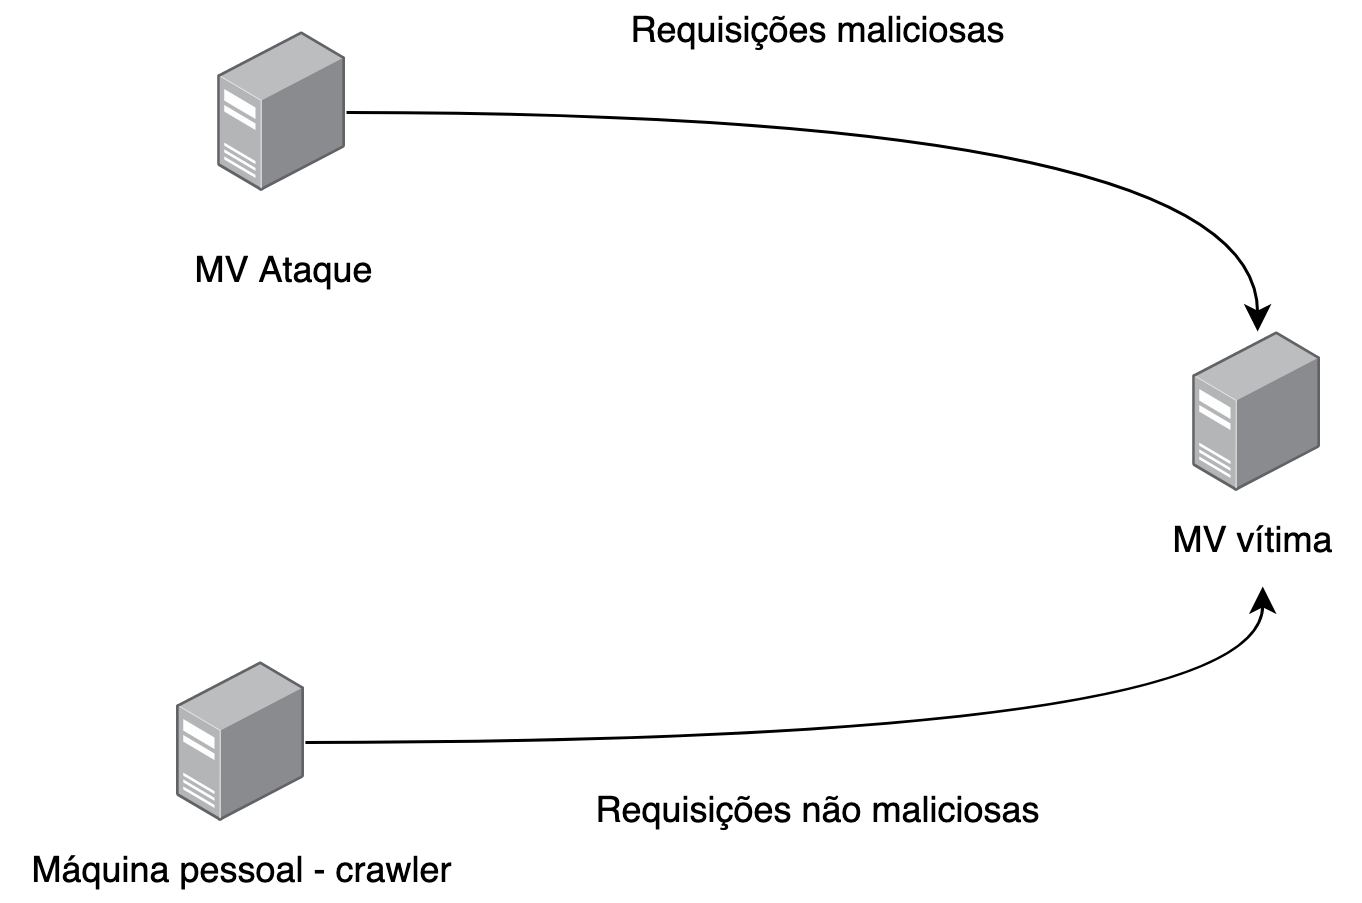
\includegraphics[width=.7\textwidth]{figuras/arquitetura_ataque.png}
    \caption{Arquitetura para simular as requisições. \label{fig:arquitetura_ataque}}    
\end{figure}

Os processos eram executados de modo que ao final, aproximadamente 10\% das requisições 
fossem maliciosas e 90\% não. Os acessos foram feitos a partir de máquinas separadas como 
mostrado na Figura \ref{fig:arquitetura_ataque}.

Na simulação o fator tempo foi arbitrariamente desconsiderado. E nos modelos ele não se mostrou 
como uma característica relevante, mas isso não descarta a possibilidade dele ser usado com uma possível
característica para classificar os dados.

\begin{figure}
    \centering
    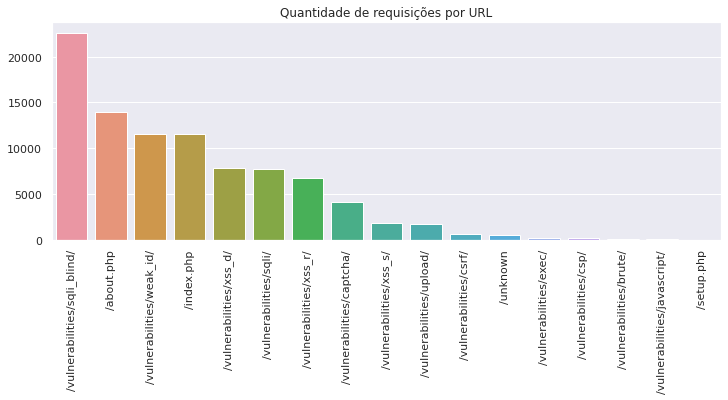
\includegraphics[width=.8\textwidth]{figuras/request_por_url.png}
    \caption{Requisições por URL. \label{fig:request_por_url}}    
\end{figure}
\begin{figure}[H]
    \centering
    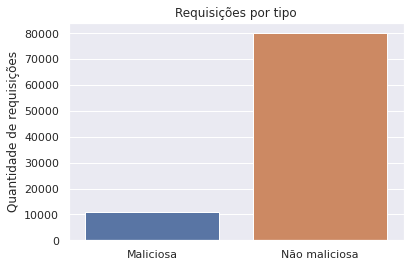
\includegraphics[width=.7\textwidth]{figuras/request_por_tipo.png}
    \caption{Requisições por tipo. \label{fig:request_por_tipo}}    
\end{figure}
\begin{figure}[H]
    \centering
    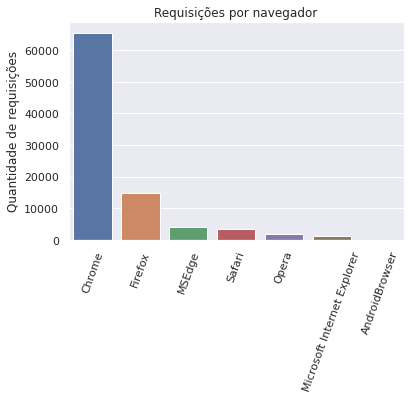
\includegraphics[width=.7\textwidth]{figuras/requisicoes_por_navegador.png}
    \caption{Requisições por navegador. \label{fig:request_por_navegador}}    
\end{figure}

As figuras \ref{fig:request_por_url}, \ref{fig:request_por_tipo} e \ref{fig:request_por_navegador} resumem 
as requisições realizadas. Nota-se que os critérios estabelecidos foram satisfeitos. Por exemplo, na
Figura \ref{fig:request_por_url} há uma quantidade maior de requisições em certas URLs, na Figura 
\ref{fig:request_por_tipo} há mais requisições não maliciosas do que maliciosas e 
na Figura \ref{fig:request_por_navegador} vemos a predominância dos navegadores Google Chrome e 
Firefox. E por fim, como 
sabíamos a origem das requisições (xsser, sqlmap ou crawler) construir a fonte da verdade para estes 
dados foi uma tarefa trivial.

\subsection{Dados reais}

Em paralelo às simulações anteriores, procuramos logs de servidores reais para que os modelos 
encontrados fossem testados e validades neles. 

Para isso entramos em contato com os autores dos artigos mencionados no Capítulo 2, e 
perguntamos quais dados foram usados em seus respectivos artigos. Jaron Fontaine, um dos autores
do artigo \cite{ref:art6} nos respondeu com os dados utilizados e eles estavam disponíveis de
maneira pública. 

Os dados indicados fazem parte de um projeto chamado The Honeynet Project \footnote{\url{https://www.honeynet.org/}}. 
Trata-se de uma organização de pesquisa 
sem fins lucrativos, que tem como objetivo pesquisar e investigar os últimos ataques e desenvolver
ferramentas open source para melhorar a segurança da internet.

Os dados faziam parte de uma competição de segurança da informação, e foram coletados da seguintes maneira:

\begin{itemize}
    \item Uma aplicação web com múltiplos servidores foi disponibilizada publicamente.
    \item Escolheu-se alguns dos servidores para subir uma versão da aplicação 
    com falhas de segurança conhecidas.
    \item Então monitorou-se a atividade nesses servidores com falhas para detectar intrusões.
\end{itemize}

Apesar dos dados serem reais, a competição tratava-se de identificar, a partir dos logs, quais requisições 
eram maliciosas e também se o ataque foi realizado com sucesso ou não. 

Nesse sentido, isso foi um desafio, dado que a fonte da verdade não era pública e a quantidade de logs 
coletados é consideravelmente grande. Então classificá-los manualmente foi necessário e para 
isso foi utilizado o script que se encontra no apêndice.

No fim, foram classificadas aproximadamente 10000 linhas e este conjunto de logs foi utilizado para validar os modelos em dados
reais.

\subsection{Estruturando os logs}

Os logs em seu formato bruto não podem ser usados como entradas para modelos de aprendizagem
de máquina, então um pré-processamento foi necessário. Por conta do padrão mencionado no  início deste capítulo, 
foi possível criar um script que os estruturasse. Abaixo um trecho de código
que foi usado nessa tarefa:

\begin{lstlisting}[language=Python]
def transformLogFileToDataframe(logFilePath, isMalicious):
    lineformat = re.compile(r"""(?P<ipaddress>\d{1,3}\.\d{1,3}\.\d{1,3}\.\d{1,3}) - - \[(?P<dateandtime>\d{2}\/[a-z]{3}\/\d{4}:\d{2}:\d{2}:\d{2} (\+|\-)\d{4})\] ((\"(GET|POST) )(?P<url>.+)(http\/[1-2]\.[0-9]")) (?P<statuscode>\d{3}) (?P<bytessent>\d+) (?P<refferer>-|"([^"]+)") (["](?P<useragent>[^"]+)["])""", re.IGNORECASE)

    logFile = open(logFilePath)

    logs_data = []

    for l in logFile.readlines():
        data = re.search(lineformat, l)

        if data is None:
            print("Falha ao fazer o parse da linha {} do arquivo {}. Pulando..".format(l, logFile))
            continue

        datadict = data.groupdict()
        datadict["malicious"] = isMalicious
        logs_data.append(datadict)

    logFile.close()

    df = pd.DataFrame(logs_data)

    df["statuscode"] = df["statuscode"].apply(int)
    df["qtd_query_params"] = df["url"].apply(quantidade_de_params_na_query)

    return df
\end{lstlisting}

No código acima, primeiro criamos uma expressão regular que irá capturar as informações de cada linha do log. 
Em seguida, abrimos o arquivo de log, aplicamos a expressão regular e em caso de sucesso, adicionamos ao 
dicionário logs\_data que irá guardar as informações de cada linha. Ao final, temos o log em um formato tabular
que pode ser usado nos modelos de aprendizagem de máquina.
\par

%!TeX root=../tese.tex
%("dica" para o editor de texto: este arquivo é parte de um documento maior)
% para saber mais: https://tex.stackexchange.com/q/78101/183146

%% ------------------------------------------------------------------------- %%
\chapter{Modelos}
\label{cap:models}

Este capitulo tem como objetivo mostrar como os modelos escolhidos e apresentar
algumas métricas nos dados simulados e reais.

Os resultados aqui apresentados foram obtidos nos notebooks do Google Colab, uma vez que 
que este foi o ambiente escolhido para compartilhar os resultados dos nosso experimentos. 

Por fim, durante a seleção dos modelos apenas os dados simulados foram usados, uma vez
que ainda não estavamos de posse dos logs reais, portanto apenas na última seção deste capítulo
mostramos a performance do modelo escolhido nos dados reais.


\subsection{Estrutura dos dados}

No final do capitulo anterior mostrou-se como os arquivos brutos de logs foram transformados
para um formato tabular, as colunas nele contidas podem ser vistos na tabela \ref{tab:exemplo_log}. 
Aqui forneceremos um dicionário do que significa cada coluna:


\begin{itemize}
    \item ipaddress: o IP do usuário que realizou a requisição.
    \item dateandtime: a data e hora em que a requisião foi realizada.
    \item url: a url requisitada.
    \item statuscode: o codigo HTTP de retorno.
    \item bytessent: quando bytes foram retornados na requisição.
    \item refferer: contém o valor do cabeçalho Refere.
    \item useragent: o agente responsável pela requisição.
    \item malicious: variável indicadora que é 1 se a requisição é maliciosa, 0 caso contrário.
\end{itemize}


\begin{sidewaystable}
\centering

\begin{tabular}{|l|l|l|l|l|l|l|l|}
\hline
    ipaddress & dateandtime & url & statuscode & bytessent & refferer & useragent & malicious \\ \hline
    192.168.0.219 & 13/May/2021:23:38:05 -0400 & /index.php & 200 & 2937 & """-""" & "Mozilla/5.0 ..." & 0 \\ \hline
    192.168.0.219 & 13/May/2021:23:38:05 -0400 & /index.php & 200 & 2937 & """-""" & "Mozilla/5.0 ..." & 0 \\ \hline
    192.168.0.219 & 13/May/2021:23:38:05 -0400 & /vulnerabilities/sqli\_blind/ & 200 & 1711 & """-""" & "Mozilla/5.0 ..." & 0 \\ \hline
    192.168.0.219 & 13/May/2021:23:38:05 -0400 & /vulnerabilities/sqli/?extraParam=... & 200 & 1675 & """-""" & "Mozilla/5.0 ..." & 0 \\ \hline
    192.168.0.219 & 13/May/2021:23:38:05 -0400 & /vulnerabilities/xss\_d/?extraParam=.... & 200 & 1839 & """-""" & "Mozilla/5.0 ..." & 1 \\ \hline
    192.168.0.219 & 13/May/2021:23:38:05 -0400 & /vulnerabilities/sqli\_blind/?extraParam.... & 200 & 1711 & """-""" & "Mozilla/5.0 ..." & 0 \\ \hline
    192.168.0.219 & 13/May/2021:23:38:05 -0400 & /about.php & 200 & 2306 & """-""" & "Mozilla/5.0 ..." & 0 \\ \hline
    192.168.0.219 & 13/May/2021:23:38:05 -0400 & /vulnerabilities/xss\_r/ & 200 & 1686 & """-""" & "Mozilla/5.0 ..." & 1 \\ \hline
\end{tabular}

\caption{Resultado final dos logs.\label{tab:exemplo_log}}

\end{sidewaystable}

De posse dessas colunas que vieram dos logs, mais 3 colunas foram criadas:

\begin{itemize}
    \item url\_sem\_query: armazena a url requisitada sem o paramêtros de consulta.
    \item qtd\_query\_params: quantidade de paramêtros encontrados na query.
    \item navegador: armazena apenas o nome do navegador presente na coluna useragent.
\end{itemize}


\subsection{Preparação dos dados}

Durante o treino/validação de todos os modelos deste capitulo, o conjunto de dados original foi divido 
em treino e teste, como explicado abaixo:

\begin{itemize}
    \item treino: dados que serão usados para treinar o modelo.
    \item teste: dados não presentes no trieno com o objetivo de verificar se o modelo generaliza bem ou não.
\end{itemize}

Outro ponto de atenção necessário é manter o desbalancemento da variável resposta (coluna malicious) nos 
conjuntos acima, dado que há mais requisições maliciosas do que não maliciosas. 

Por fim, dados categóricos foram transformados em números usando a técnica de OneHotEncode. Este e o item
anterior foram feitos com o auxilio dos utilitários de pré-processamento de dados do scikit-learn e do Apache Spark.

\subsection{Modelo base}

O modelo de florestar aleatória foi escolhido como modelo base. Essa escolha se deve ao fato dos autores 
terem uma familiaridade com ele de projetos anteriores. 

Para avaliar o modelo, as colunas abaixo foram escolhidas de maneira árbitrário, ja que neste ponto 
queriamos saber se modelos de árvores resolveriam nosso problema.

\begin{itemize}
    \item statuscode
    \item navegador
    \item qtd\_query\_params
    \item bytessent
\end{itemize}


Com este modelo e as colunas mencionadas conseguimos uma acurácia de 1 nos dados de teste. Surprendente, pois 
não esperavamos esse resultado na primeira tentativa, dado que se trata de um modelo base, logo suspeitamos 
que o modelo estava sobre ajustado nos dados. 

Para ter uma intuição melhor de como o modelo estava realizando a classificação, optamos por experimentar 
o modelo de árvore de decisão, dado que depurar-lo é possível.

\subsection{Depurando o modelo - árvore de decisão}

As mesmas colunas da seção anterior foram usadas para treinar uma árvore de decisão, e novamente
o modelo teve uma acurácia de 1 nos dados de treino e teste. 

Para entender como a classificação está sendo realizada, exibimos árvore final na imagem \ref{fig:primeira_arvore}. Nesse sentido, 
como os dados parassaram por um pré-processamento de OneHotEncoder vale mencionar o que significam cada índica em X:

\begin{itemize}
    \item X[0] e X[1]: é a coluna statuscode.
    \item X[3] até X[9]: indicam o navegador que foi utilizado.
    \item X[10]: é a coluna qtd\_query\_params
    \item X[11]: é a coluna bytessent
\end{itemize}

\begin{figure}
    \centering
    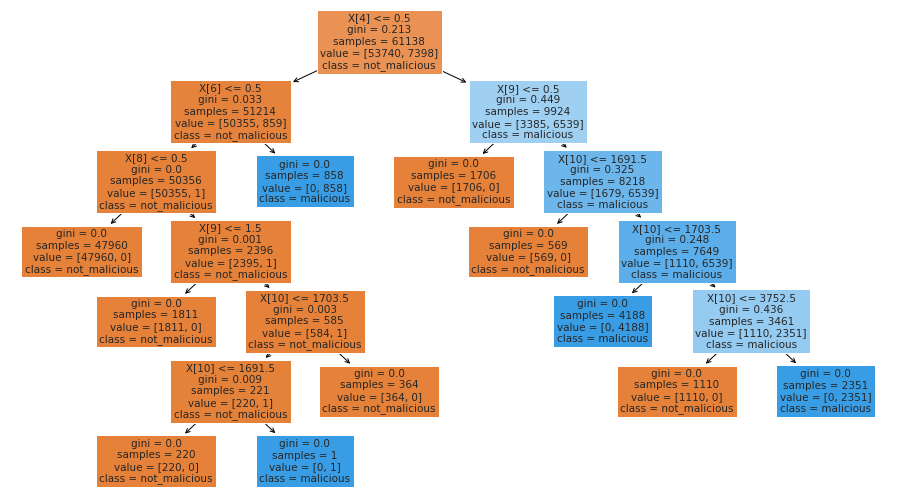
\includegraphics[width=.9\textwidth]{figuras/primeira-arvore.png}
    \caption{Primeira árvore de decisão. \label{fig:primeira_arvore}}    
\end{figure}

Vemos que a árvore esta usando majoritariamente os dados da coluna navegador 
para realizar a classifição, o que não faz sentido, dado que esse dado foi simulado e o 
navegador não tem nenhuma relação com os ataques. Então removemos essa coluna da entrada 
e o resultado está na imagem \ref{fig:segunda_arvore}.


\begin{figure}
    \centering
    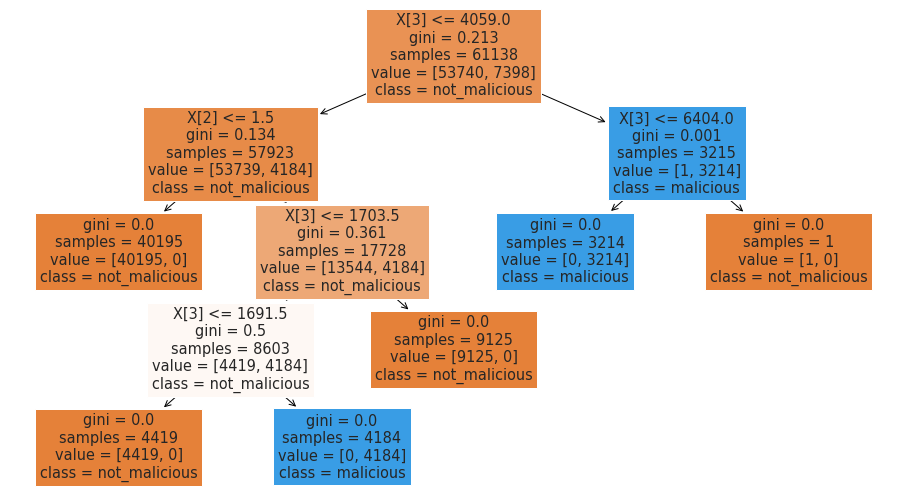
\includegraphics[width=.9\textwidth]{figuras/segunda_arvore.png}
    \caption{Segunda árvore de decisão. \label{fig:segunda_arvore}}    
\end{figure}

Esta versão já nos pareceu mais sólida pois ela utiliza a quantidade de paramêtros na query 
e a quantidade bytes enviados para o cliente, o que está relacionado com os ataques. Além disso,
também atingiu uma acurácia de 1.

\subsection{Escolha do modelo e considerações}

Dado o que foi apresentado nas seções anteiories, escolhemos o modelo de árvore de decisão com as colunas
abaixo para realizar os experimentos e valida-lo em dados reais. 

\begin{itemize}
    \item statuscode
    \item qtd\_query\_params
    \item bytessent
\end{itemize}

Outros modelos mais complexos, como redes neurais ou xgboost, não foram considerados pois o 
objetivo deste trabalho é usar-lo em computadores onde os recursos, como memória e disco, são
limitados portanto favorecendo modelos mais simples como o escolhido.

Também vale notar que características dos logs específicas a ataques XSS e SQL Injection, como 
verificar a existência de uma consulta SQL na url, não foram criadas pois as colunas padrões 
do log foram suficientes para conseguir uma acurácia considerada boa.

\subsection{Testes em dados reais}

De posse dos dados reais mencionados na seção 4.2.2, executamos o modelo escolhido neles e atingimos 
uma acurácia de aproximadamente 0.93 nos dados de teste, o que consideramos próximos dos resultados 
obtidos nos artigos do capítulo 2, porém com um modelo mais simples. Portanto, definitivamente definitivamente
seguimos com ele nos experimentos.

\par

%!TeX root=../tese.tex
%("dica" para o editor de texto: este arquivo é parte de um documento maior)
% para saber mais: https://tex.stackexchange.com/q/78101/183146

%% ------------------------------------------------------------------------- %%
\chapter{Análise de resultados}
\label{cap:results}

Aqui vamos analisar os resultados
\par

%!TeX root=../tese.tex
%("dica" para o editor de texto: este arquivo é parte de um documento maior)
% para saber mais: https://tex.stackexchange.com/q/78101/183146

%% ------------------------------------------------------------------------- %%
\chapter{Conclusão}
\label{cap:conclusao}

O modelo de árvore de decisão provou-se eficaz na tarefa de detectar intrusões
a partir dos logs. Além disso, não foi necessária nenhuma característica específica
dos ataques para atingir uma boa acurácia.

Para treinar o modelo, conclui-se que é preferível optar por um computador com 
especificações similares ao Macbook utilizado, dado o consumo de CPU que foi
observado.

Por fim, para a classificação o Raspberry Pi pode ser utilizado quando o fator 
tempo não for um impeditivo, pois foi observado que ele demora em média 6 vezes 
mais para classificar do que o Macbook.
\par

%!TeX root=../tese.tex
%("dica" para o editor de texto: este arquivo é parte de um documento maior)
% para saber mais: https://tex.stackexchange.com/q/78101/183146

%% ------------------------------------------------------------------------- %%
\chapter{Avaliação pessoal e crítica}
\label{cap:avaliacao_pessoal}

O tema deste trabalho foi escolhido principalmente por dois motivos:

\begin{itemize}
    \item Aprofundar no tema de aprendizagem de máquina.
    \item Aprender mais sobre computação distribuída e Apache Spark.
\end{itemize}

O primeiro foi atingido, pois o contato e desenvolvimento nesse tema que eu tive
foi muito produtivo e me ajudou em muito.

O segundo, foi atendido parcialmente, dado que o contato com Apache Spark ocorreu,
contudo, durante os experimentos, o segundo Raspberry Pi queimou e a oportunidade de 
trabalhar com aprendizagem de máquina de maneira distribuída não ocorreu como eu 
esperava. Porém fica o aprendizado de estar preparado para qualquer adversidade em
trabalhos futuros.

A crítica principal a este trabalho foi ter utilizado o Apache Spark em um único nó 
de Raspberry Pi, pois esse não é o objetivo da ferramenta, contudo o experimento e 
script já estavam prontos e alterá-los nos tomaria tempo que não dispunhamos. 

Por fim, durante o trabalho o conhecimento das seguintes disciplinas foi utilizado: sistemas
operacionais para entender como utilizar da melhor maneira cada computador, ciência e engenharia
de dados que mostrou ferramentas para processamento de dados, aprendizagem de máquina onde os 
modelos foram expostos de maneira mais formal, língua portuguesa para a escrita desta monografia
e as disciplinas de estatística para entender melhor os modelos, além de ajudar a formalizar os 
experimentos. Por fim, a prática adquirida no grupo de extensão  BeeData, um dos vários grupos 
de extensão do IME-USP, mostrou-se bastante útil neste trabalho.

\par
